\chapter{ Introducción Específica } % Main chapter title
%----------------------------------------------------------------------------------------
%	SECTION 1
%----------------------------------------------------------------------------------------
\section{ Que es el Galvanizado de un PCB? }

El proceso de galvanizado consiste en adherir a un objeto metálico una delgada capa de otro metal, de unos pocos micrones de espesor. Este material le otorga mejores propiedades al objeto como ser conductividad eléctrica, mayor resistencia mecánica o resistencia a la corrosión. 
Los métodos para lograrlos pueden ser diversos entre los mas comunes son con un baño químico y por electrolisis.
La forma utilizada en los PCBs (Printed Circuit Board o placa de circuito integrado) es a través de la electrolisis del objeto dentro de una solución con sales metálicas, mas una fuente continua de bajo voltaje y muy alta corriente, mas bloques del metal necesario para el galvanizado. 
La figura \ref{fig:galvanizado_electrolitico} es un diagrama simplificado de este proceso, aquí el ánodo es de cobre y el cátodo es el PCB a galvanizar.

\begin{figure}[h]
	\centering
	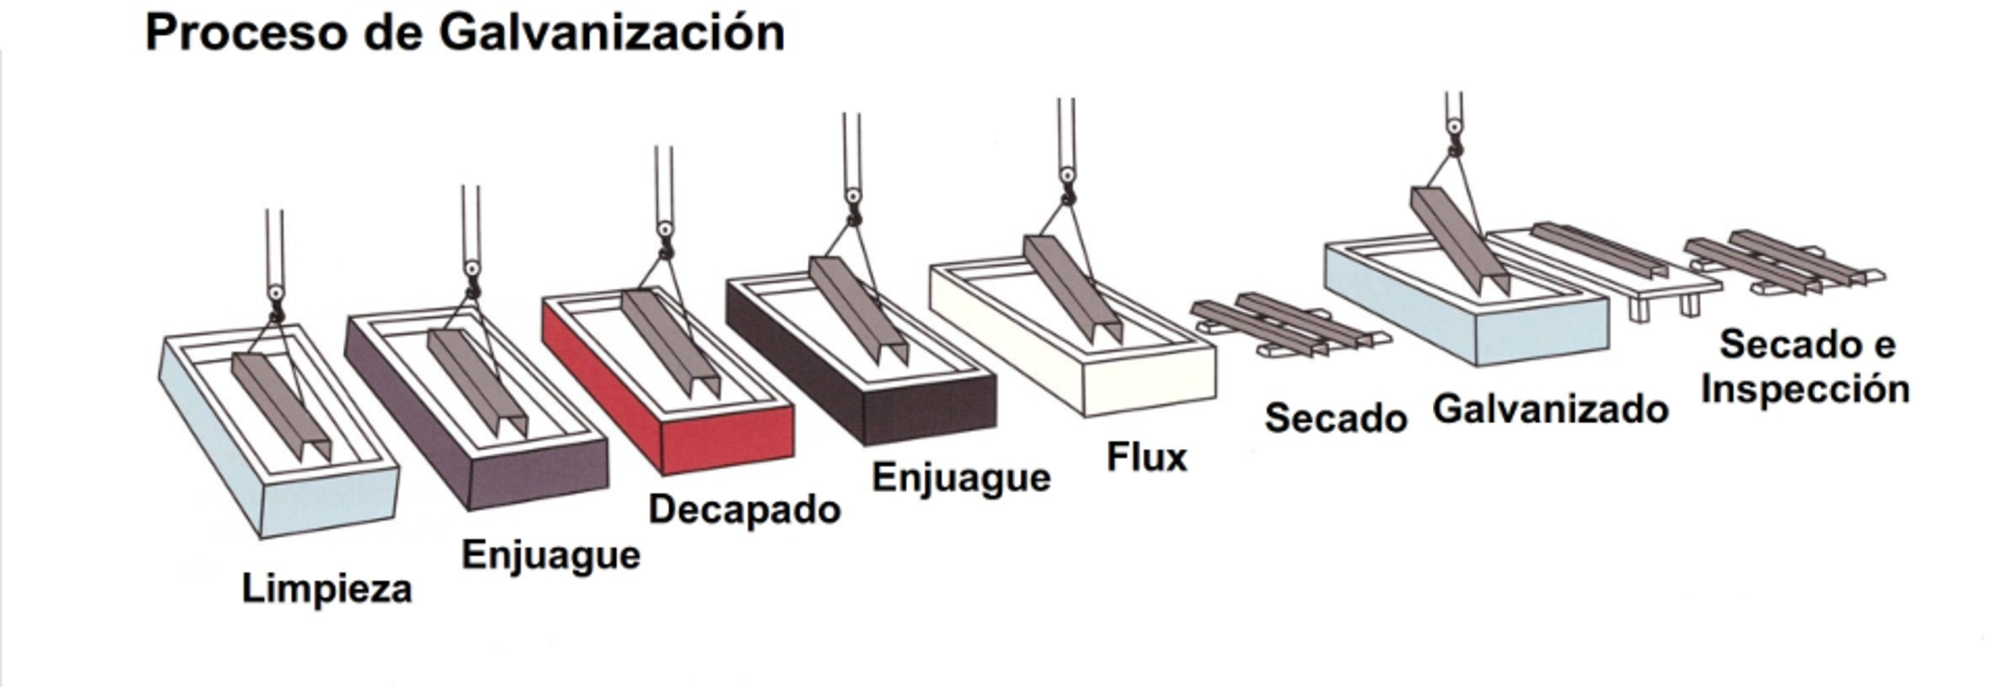
\includegraphics[width=.9\textwidth]{Figures/Cap_2/diagrama_galvanizado_basico}
	\caption{Proceso electrolítico con fuente continua.}
	\label{fig:galvanizado_electrolitico}
\end{figure}


\subsection{ Proceso de Galvanizado por Electrolisis }

En la fabricación de PCBs se parte de un material base de sustrato de laminas epoxi Fr4 revestido con laminas de cobre. Este debe ser sometido previo a realizar la electrolisis en si, a una sucesión de baños químicos para limpiar y homogeneizar toda las partes metálicas de superficie. El proceso es repetido con variantes del metal galvánico para lograr el circuito final. 
En la Figura \ref{fig:diagrama_proceso} se resumen los pasos de forma simplificada, en el proceso de PCB se utilizan mas de 10 etapas. 

\begin{figure}[h]
	\centering
	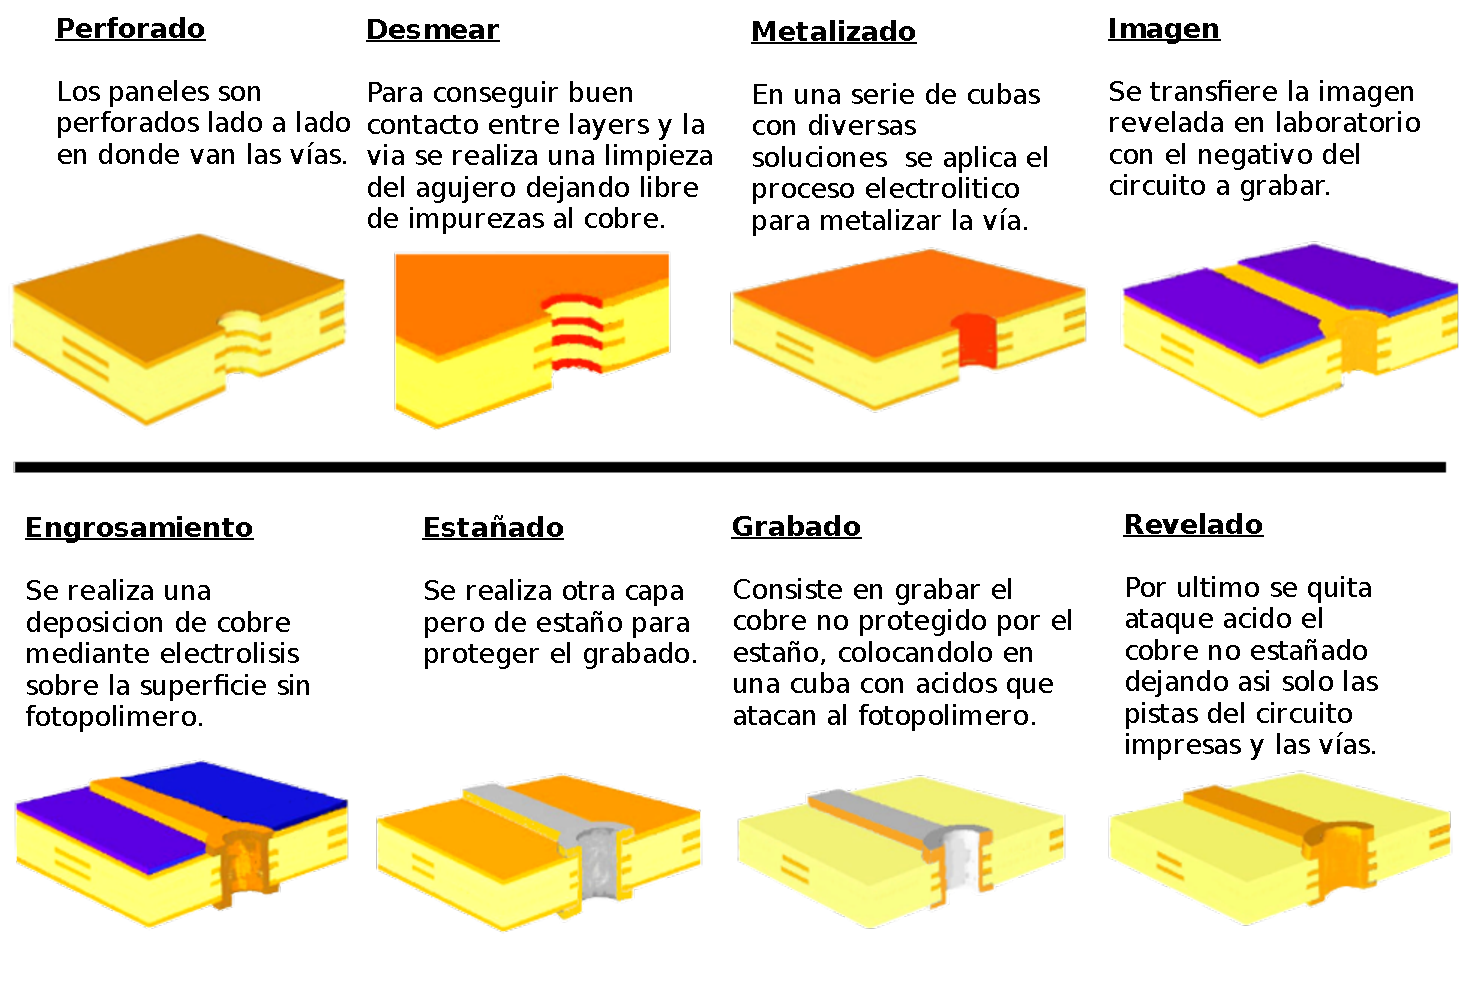
\includegraphics[width=1.0\textwidth]{Figures/Cap_2/diagrama_galvanizado_completo}
	\caption{Diagrama simplificado de las etapas.}
	\label{fig:diagrama_proceso}
\end{figure}

En este caso de estudio nos focalizamos en el primero que se usa tanto para metalizar las vías entre capas (previamente perforadas) como para engrosar el cobre base que originara las pistas del circuito. La figura \ref{fig:galvanizado_pcb} muestra el resultado final de un PTH (Plated Through Hole o agujero pasante metalizado) o simplemente vía, en un PCB.

\begin{figure}[h]
	\centering
	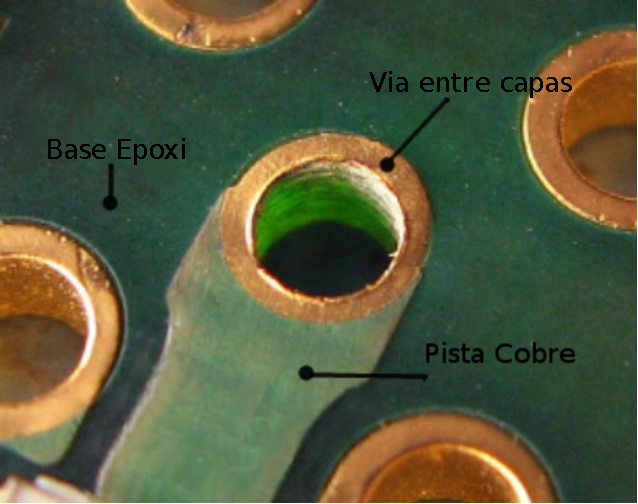
\includegraphics[width=.5\textwidth]{Figures/Cap_2/galvanizado_pcb}
	\caption{Vía entre capas galvanizada en un PCB}
	\label{fig:galvanizado_pcb}
\end{figure}

\section{ Parámetros críticos del galvanizado }

En el proceso de galvanización de PCBs el control de ciertos parámetros físicos-químicos en cada una de las etapas es fundamental para garantizar la uniformidad y calidad del baño de cobre. 

En las diferentes bateas de la linea de galvanizado es necesario controlar, según cada etapa uno o algunos de los siguientes parámetros físicos-químicos del proceso:
\begin{itemize}
	\item Temperatura.
	\item Nivel de líquidos.
	\item Conductividad o concentración de iones.
	\item Corriente entregada (electrolisis).
	\item Inyección de aire.
\end{itemize}

Actualmente en la linea de galvanizado los operadores solo cuentan con su experiencia y con el soporte de instrumental de medición básico, para usar en algunas las etapas de la linea. Para saber cuando una etapa esta realizada correctamente es necesario tener información precisa y detallada para garantizar el resultado. Esto es causante de que el producto final muchas veces no tenga una calidad estándar y que no se puedan prevenir fallas en proceso a tiempo.

\subsection{ Fallas en la galvanización de PCBs }

En la producción de PCBs el resultado final correcto es aquel donde el espesor del baño metálico es uniforme en toda la cavidad. Cuando este proceso no ocurre correctamente se originan distintas fallas, donde las más comunes son:
\begin{itemize}
	\item Vías sin galvanizar.
	\item vías obstruidas por exceso de cobre.
	\item Laminado no uniforme de metal cobre.
	\item Micro cortes del cobre y puntos de no conductividad.
\end{itemize}

En la Figura \ref{thr_incorrecto_perfil} se observan las distintos grosores de cobre con vías mal galvanizadas en función de su ubicación en el sustrato del PCB y la cercanía al ánodo de cobre.

\begin{figure}[h]
	\centering
	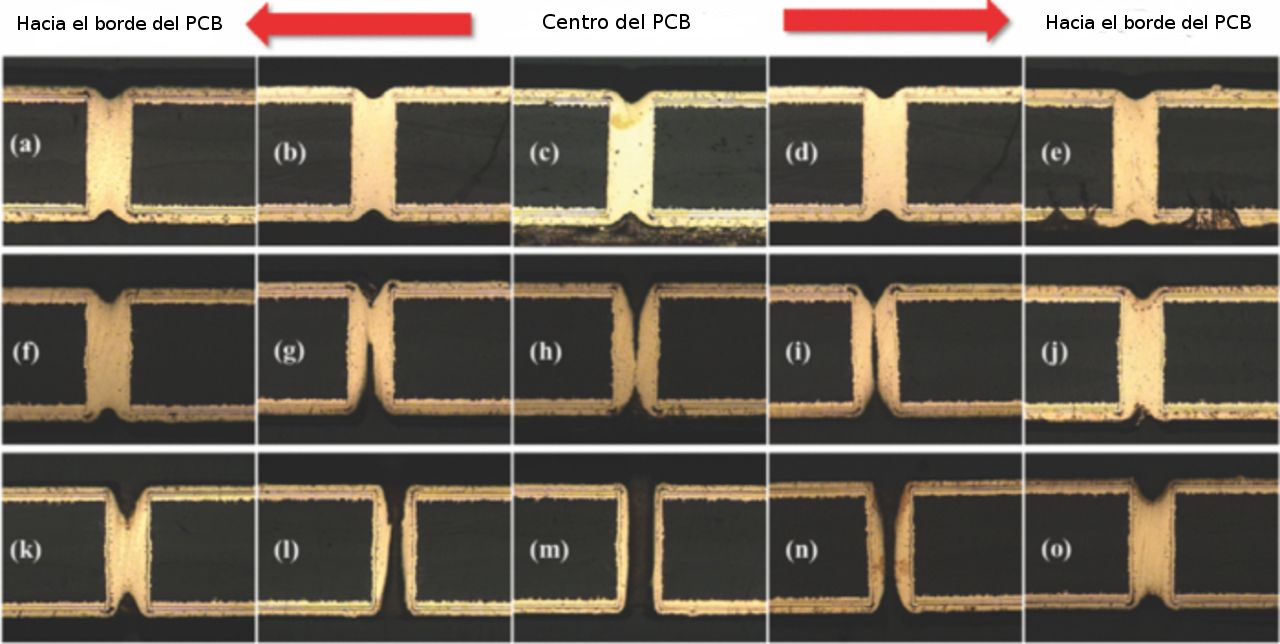
\includegraphics[width=.9\textwidth]{Figures/Cap_2/through_hole_perfil_fallado}
	\caption{Perfil de vías según la ubicación relativa en los sustratos y el los cátodos.}
	\label{fig:thr_incorrecto_perfil}
\end{figure}

En la figura \ref{thr_incorrecto_perfil} se observa los problemas originados por la mala preparación previa de las superficies metálicas del sustrato, originado puntos sin continuidad o circuitos abiertos que lo volverán no aptos para la producción de circuitos.

\begin{figure}[h]
	\centering
	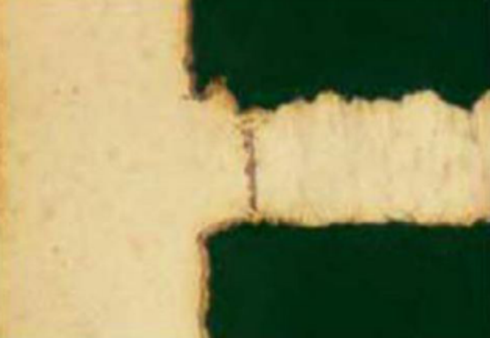
\includegraphics[width=.5\textwidth]{Figures/Cap_2/etchback_thr_incorrecto_perfil}
	\caption{ Las capas de cobre se alejan del borde del orificio.}
	\label{fig:thr_incorrecto_perfil}
\end{figure}

\section{ Determinación de la solución } 

A fin de lograr determinar detalles de la arquitectura del sistema desarrollado es necesario definir y determinar casos de uso, requerimientos técnicos y definiciones generales originados por la nueva planta, su operación y las necesidades del cliente. 

\subsection{ Definiciones Generales }

Debido a que la linea cuenta con varias etapas en forma consecutiva independientes entre si pero con características similares, se determino implementar un prototipo capaz de procesar el conjunto de parámetros del proceso y capaz de interactuar con los distintos usuarios del entorno.

El sistema debería de funcionaria en modo predeterminado según los distintos escenarios posibles dentro de las etapas del proceso. De esta manera con un mismo hardware mas los sensores y actuadores necesarios, se puede hacer supervisión y control en las partes del proceso que se crean necesarias.

En una etapa posterior luego de la validación del prototipo el cliente desarrollaría un hardware a medida para usar en su planta. El mismo seria producido en las cantidades necesarias según el numero de etapas que se determinaran. Por ultimo estos distintos módulos deberían funcionar de manera independiente entre si.


\subsection{ Casos de Uso }

Se definieron los casos de uso del sistema para determinar como se vincularía el sistema con los distintos usuario, en función del modo de funcionamiento posible. Estos quedan entonces predeterminados por los escenarios posibles que se puede originar en la operación de la linea.
Los casos mas relevantes son:
\begin{enumerate}
	\item Puesta en alta y configuración del dispositivo, usado por personal técnico.
	\item Operación en modo de funcionamiento 1, usado por el operario y el técnico.
	\item Operación en modo de funcionamiento 2, usado por el operario y el técnico.
\end{enumerate}

En la Figuras \ref{fig:casoUsoAlta} y \ref{fig:casodeUso1y2} se notan las interacciones entre los distintos submódulos del sistema en función de los casos de usos y los usuarios vinculados.

\begin{figure}[h!]
	\centering
	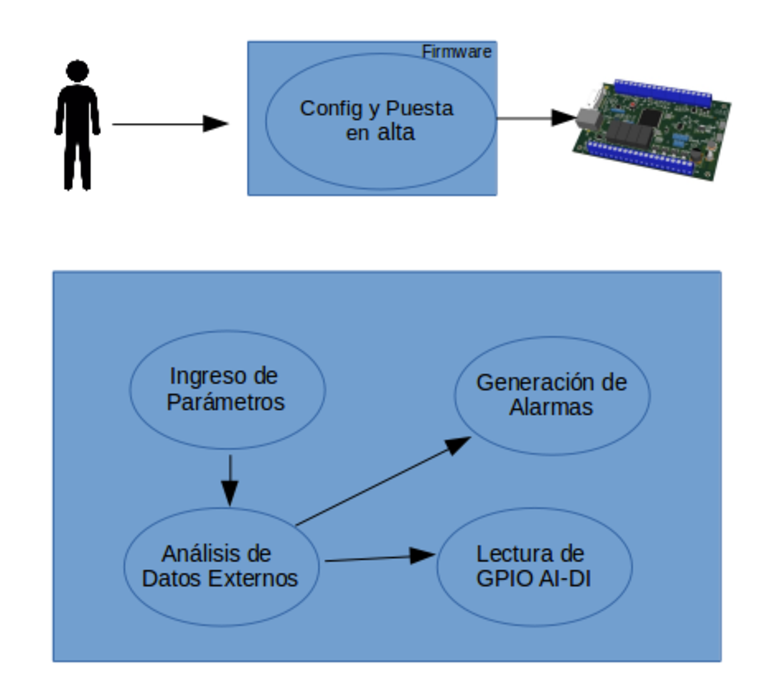
\includegraphics[width=.7\textwidth]{Figures/Cap_2/caso_uso_Alta_UML}
	\caption{Diagrama UML caso de uso de puesta en alta.}
	\label{fig:casoUsoAlta}
\end{figure}

La puesta en alta es el momento en que se determinan a través de la interface terminal HMI (Humman Machine Interface o interfase hombre maquina) las parámetros a medir y configuraciones de los puertos del hardware.

\begin{figure}[h!]
	\centering
	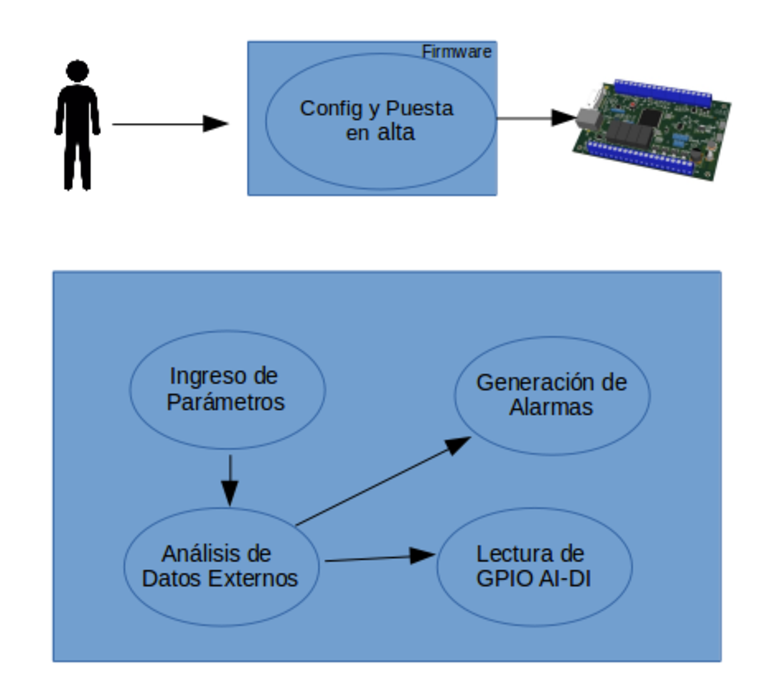
\includegraphics[width=.7\textwidth]{Figures/Cap_2/caso_uso_1y2_UML}
	\caption{Diagrama UML de casos de uso Modo 1 y 2.}
	\label{fig:casodeUso1y2}
\end{figure}

Los modos 1 y 2 se refieren a dos configuraciones estandars y predefinidas que se crearon a partir de los escenarios mas comunes en las que se utilizaría el prototipo a fin de simplificar la puesta en marcha en campo.
En el apéndice \ref{AppendixA} se detallan la secuencias involucradas en cada una de los casos de uso.

\subsection{ Requerimientos Funcionales y no Funcionales }
\label{subsec:Requerimientos}

A fin de no ahondar con detalles técnicos el documento a lista completa con los requerimientos se pueden ver en el anexo \ref{AppendixC}. Cabe mencionar que el mismo se originó previamente en la materia Taller de Trabajo Final en el posgrado.
\\
En función de estos se propuso implementar el proyecto sobre una plataforma EDU-CIAA en conjunto con una placa de interfaz hecha a medida. 







